
%----------------------------------------------------------------------------------------
%	Machine Learning Assignment Template
%----------------------------------------------------------------------------------------

\documentclass[11pt]{scrartcl}
\newcommand*\student[1]{\newcommand{\thestudent}{{#1}}}

%----------------------------------------------------------------------------------------
%	INSERT HERE YOUR NAME
%----------------------------------------------------------------------------------------

\student{Omenetti Matteo, Ravi Srinivasan}

%----------------------------------------------------------------------------------------
%	PACKAGES AND OTHER DOCUMENT CONFIGURATIONS
%----------------------------------------------------------------------------------------

\usepackage[utf8]{inputenc} % Required for inputting international characters
\usepackage[T1]{fontenc} % Use 8-bit encoding
\usepackage[sc]{mathpazo}
\usepackage{caption, subcaption}
\usepackage{hyperref}
\usepackage{inconsolata}

\usepackage[english]{babel} % English language hyphenation
\usepackage{amsmath, amsfonts} % Math packages
\usepackage{listings} % Code listings, with syntax highlighting
\usepackage{graphicx} % Required for inserting images
\graphicspath{{Figures/}{./}} % Specifies where to look for included images (trailing slash required)
\usepackage{float}
\usepackage{mathtools}


%----------------------------------------------------------------------------------------
%	DOCUMENT MARGINS
%----------------------------------------------------------------------------------------

\usepackage{geometry} % For page dimensions and margins
\geometry{
	paper=a4paper, 
	top=2.5cm, % Top margin
	bottom=3cm, % Bottom margin
	left=3cm, % Left margin
	right=3cm, % Right margin
}

%----------------------------------------------------------------------------------------
%	SECTION TITLES
%----------------------------------------------------------------------------------------

\usepackage{sectsty}
%\sectionfont{\vspace{6pt}\centering\normalfont\scshape}
\subsectionfont{\normalfont\bfseries} % \subsection{} styling
\subsubsectionfont{\normalfont\itshape} % \subsubsection{} styling
\paragraphfont{\normalfont\scshape} % \paragraph{} styling

%----------------------------------------------------------------------------------------
%	HEADERS AND FOOTERS
%----------------------------------------------------------------------------------------

\usepackage{scrlayer-scrpage}
\ofoot*{\pagemark} % Right footer
\ifoot*{\thestudent} % Left footer
\cfoot*{} % Centre footer

%----------------------------------------------------------------------------------------
%	TITLE SECTION
%----------------------------------------------------------------------------------------

\title{	
	\normalfont\normalsize
	\textsc{Machine Learning for Health Care\\%
	ETH Zürich}\\
	\vspace{25pt}
	\rule{\linewidth}{0.5pt}\\
	\vspace{20pt}
	{\huge Project 1}\\
	\vspace{12pt}
	\rule{\linewidth}{1pt}\\
	\vspace{12pt}
}

\author{\LARGE \thestudent}

\date{\normalsize\today}

\begin{document}

\maketitle
\newpage

\section{Introduction}
The following report is... tutto trainato su colabpro tutto riproducibile e tutti gli h5 files.

%%%%%%%%%%%%%%%%%%%%%%%%%%%%%%%%%%%%% VANILLA CNN %%%%%%%%%%%%%%%%%%%%%%%%%%%%%%%%%%%%%%%%%%%%%%%%%%
\section{Convolutional Neural Network (CNN)}
For the vanilla CNN, a smaller model compared to the one provided as a baseline was built. The reason behind this shallower architecture is that we were curious to understand whether the decreased training cost would also result in a statistically relevant decrease in performance. However, as will be reported in the two subsections below this is not the case. 

%%%%%%% MIT %%%%%%%
\subsection{MIT\_BIH}
The model on the Mit\_Bih dataset achieves a test accuracy score of 0.981, taking around 6 minutes to train with the GPU offered by ColabPro. This model was trained with the option to reduce the learning rate on plateau for 33 epochs before early stopping kicked in.
As image \ref{fig:cnn_mit_three} and the reported accuracy show the performance of this shallower model are very close to the baseline model (accuracy 0.985) , that instead takes more than 7 minutes to train on the same GPU.
\begin{figure}[htp]
\centering
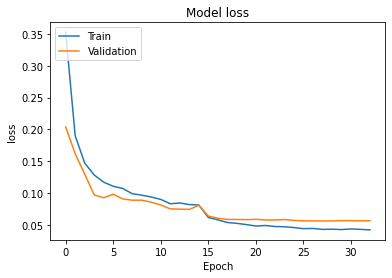
\includegraphics[width=.3\textwidth]{../models_performance_graphs/mit/CNN_mit_train_validation.png}\hfill
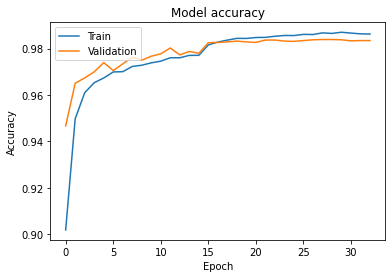
\includegraphics[width=.3\textwidth]{../models_performance_graphs/mit/cnn_mit_train_val_acc.png}\hfill
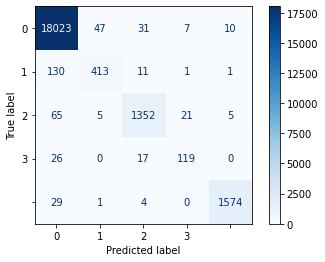
\includegraphics[width=.3\textwidth]{../models_performance_graphs/mit/cnn_mit_confusion.png}
\caption{(left) train and validation loss of the vanilla CNN for the Mit\_bih dataset. \\ (center) train and validation accuracy of the vanilla CNN for the Mit\_bih dataset. \\(right) confusion matrix of the vanilla CNN for the Mit\_bih dataset}
\label{fig:cnn_mit_three}
\end{figure}

%%%%%%% PTB %%%%%%%
\subsection{PTB}
The model on the PTB dataset achieves a test accuracy score of 0.982, taking around 1 minute to train with the GPU offered by ColabPro. 
As image \ref{fig:cnn_ptb_three} and the reported accuracy show, the performance of this shallower model is very close to the baseline model (accuracy 0.991).
The AURPRC and AUROC curves can be found in image \ref{fig:cnn_ptb_two}
\begin{figure}[htp]
\centering
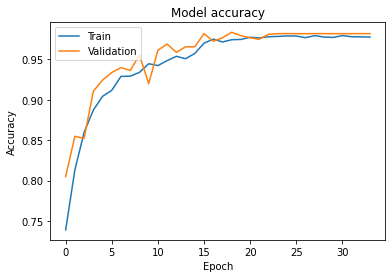
\includegraphics[width=.30\textwidth]{../models_performance_graphs/ptb/cnn_ptb_accuracy.png}\hfill
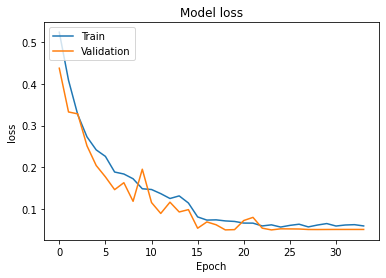
\includegraphics[width=.30\textwidth]{../models_performance_graphs/ptb/cnn_ptb_loss.png}\hfill
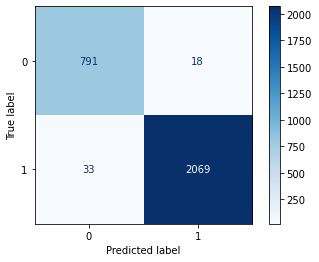
\includegraphics[width=.30\textwidth]{../models_performance_graphs/ptb/cnn_ptb_confusion.png}\hfill
\caption{(left) train and validation loss of the vanilla CNN for the PTB dataset. \\ (center) train and validation accuracy of the vanilla CNN for the PTB dataset. \\(right) confusion matrix of the vanilla CNN for the PTB dataset}
\label{fig:cnn_ptb_three}
\end{figure}

\begin{figure}[htp]
\centering
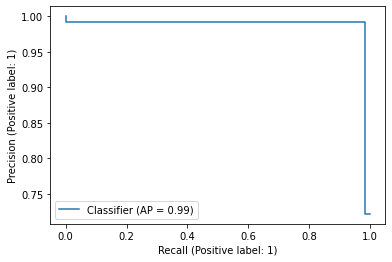
\includegraphics[width=.50\textwidth]{../models_performance_graphs/ptb/cnn_ptb_auprc.png}\hfill
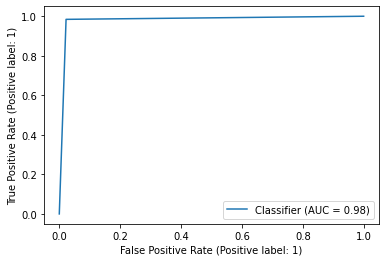
\includegraphics[width=.50\textwidth]{../models_performance_graphs/ptb/cnn_ptb_auroc.png}\hfill
\caption{(left) AURPC curve of the vanilla CNN for the PTB dataset. \\ (right) AUROC curve of the vanilla CNN for the PTB dataset}
\label{fig:cnn_ptb_two}
\end{figure}



%%%%%%%%%%%%%%%%%%%%%%%%%%%%%%%%%%%%% RES NET %%%%%%%%%%%%%%%%%%%%%%%%%%%%%%%%%%%%%%%%%%%%%%%%%%
\section{CNN with Residual Blocks}
For this task, we designed a CNN architecture very similar to ResNet. This is the model that achieves the best performance.
%%%%%%% MIT %%%%%%%
\subsection{MIT\_BIH}
This model on the Mit\_Bih dataset, achives an accuracy of 0.988. The training curves and confusion matrix are summarized in image \ref{fig:res_mit_three}.
\begin{figure}[htp]
\centering
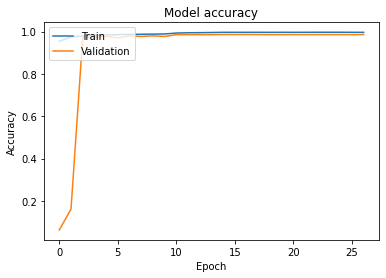
\includegraphics[width=.30\textwidth]{../models_performance_graphs/mit/res_net_mit_accuracy.png}\hfill
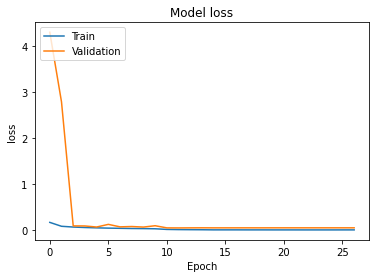
\includegraphics[width=.30\textwidth]{../models_performance_graphs/mit/res_net_mit_loss.png}\hfill
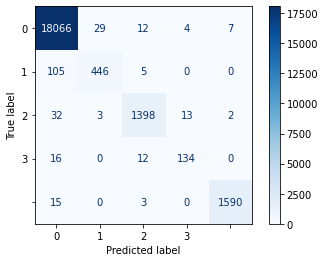
\includegraphics[width=.30\textwidth]{../models_performance_graphs/mit/res_net_mit_confusion.png}
\caption{(left) train and validation loss of the CNN with residual blocks for the Mit\_bih dataset. \\ (center) train and validation accuracy of the CNN with residual blocks for the Mit\_bih dataset. \\(right) confusion matrix of the CNN with residual blocks for the Mit\_bih dataset}
\label{fig:res_mit_three}
\end{figure}

%%%%%%% PTB %%%%%%%
\subsection{PTB}
This model on the PTB dataset, achives an accuracy of 0.986. The training AUROC, AUPRC curves and confusion matrix  are summarized in images \ref{fig:res_ptb_three} and \ref{fig:res_ptb_two}
\begin{figure}[htp]
\centering
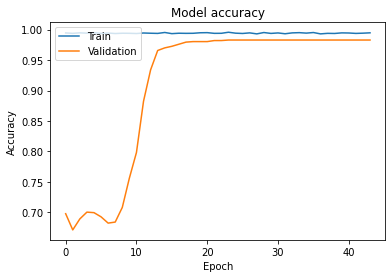
\includegraphics[width=.30\textwidth]{../models_performance_graphs/ptb/res_net_ptb_accuracy.png}\hfill
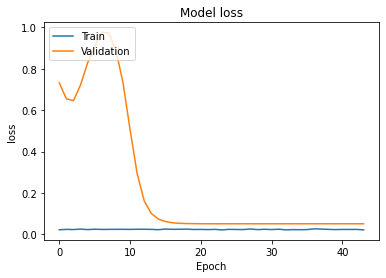
\includegraphics[width=.30\textwidth]{../models_performance_graphs/ptb/res_net_ptb_loss.png}\hfill
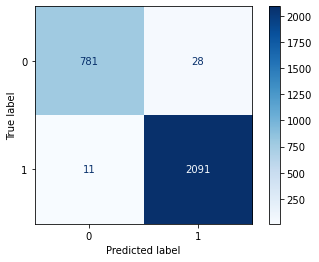
\includegraphics[width=.30\textwidth]{../models_performance_graphs/ptb/res_net_ptb_confusion.png}
\caption{(left) train and validation loss of the CNN with residual blocks for the PTB dataset. \\ (center) train and validation accuracy of the CNN with residual blocks for the PTB dataset. \\(right) confusion matrix of the CNN with residual blocks for the PTB dataset}
\label{fig:res_ptb_three}
\end{figure}

\begin{figure}[htp]
\centering
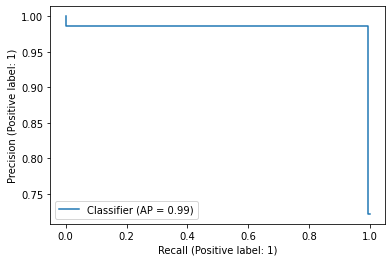
\includegraphics[width=.50\textwidth]{../models_performance_graphs/ptb/res_net_ptb_auprc.png}\hfill
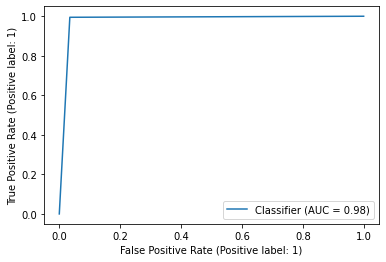
\includegraphics[width=.50\textwidth]{../models_performance_graphs/ptb/res_net_ptb_auroc.png}\hfill
\caption{(left) AURPC curve of the CNN with residual blocks for the PTB dataset. \\ (right) AUROC curve of the CNN with residual blocks for the PTB dataset}
\label{fig:res_ptb_two}
\end{figure}




%%%%%%%%%%%%%%%%%%%%%%%%%%%%%%%%%%%%% TRANSFORMER %%%%%%%%%%%%%%%%%%%%%%%%%%%%%%%%%%%%%%%%%%%%%%%%%%
\section{Transformer}
This model consists of three transformers encoder blocks, stacked on top of each other with a standard CNN at the end. This model is very heavy to train. Without ColabPro the training for the Mit\_Bih dataset is around 16hours on the TPU.  Using ColabPro, the amount of time required to train the model decreases drastically. Overall, its performance is not great if compared to the other much lighter models, therefore it is not recommended to use this model for these specific tasks. Moreover, this model is also significantly slower than all of the other models at prediction time.
%%%%%%% MIT %%%%%%%
\subsection{MIT\_BIH}
This model on the Mit\_Bih dataset, achives an accuracy of 0.976. The training curves and confusion matrix are summarized in image \ref{fig:transformer_mit_three}.
\begin{figure}[htp]
\centering
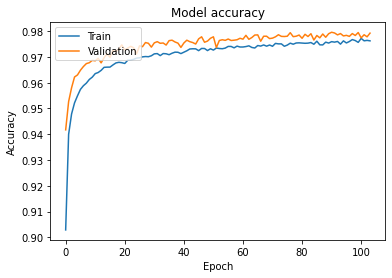
\includegraphics[width=.30\textwidth]{../models_performance_graphs/mit/transformer_mit_accuracy.png}\hfill
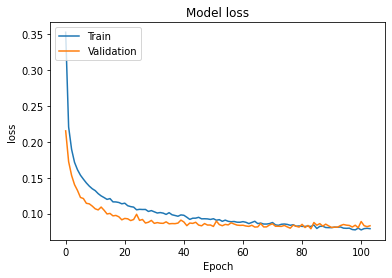
\includegraphics[width=.30\textwidth]{../models_performance_graphs/mit/transformer_mit_loss.png}\hfill
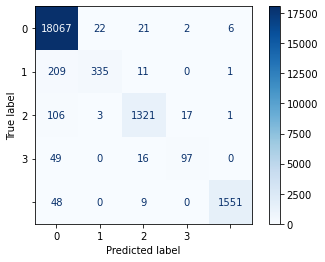
\includegraphics[width=.30\textwidth]{../models_performance_graphs/mit/transformer_mit_confusion.png}
\caption{(left) train and validation loss of the transformer for the Mit\_bih dataset. \\ (center) train and validation accuracy of the transformer for the Mit\_bih dataset. \\(right) confusion matrix of the transformer for the Mit\_bih dataset}
\label{fig:res_mit_three}
\end{figure}

%%%%%%% PTB %%%%%%%
\subsection{PTB}
This model on the PTB dataset, achives an accuracy of 0.968. The training AUROC, AUPRC curves and confusion matrix  are summarized in images \ref{fig:tranformer_ptb_three} and \ref{fig:transformer_ptb_two}
\begin{figure}[htp]
\centering
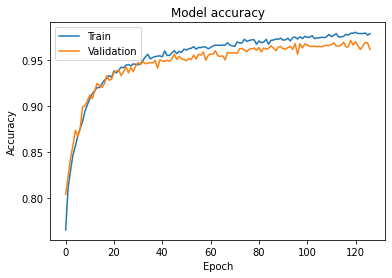
\includegraphics[width=.30\textwidth]{../models_performance_graphs/ptb/transformer_ptb_accuracy.png}\hfill
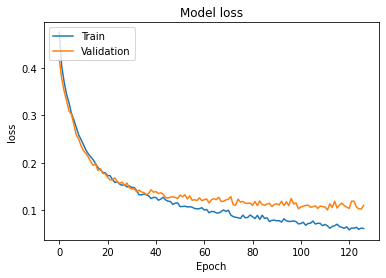
\includegraphics[width=.30\textwidth]{../models_performance_graphs/ptb/transformer_ptb_loss.png}\hfill
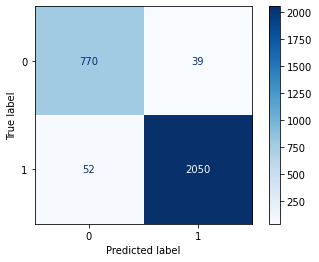
\includegraphics[width=.30\textwidth]{../models_performance_graphs/ptb/transformer_ptb_confusion.png}
\caption{(left) train and validation loss of the transformer for the PTB dataset. \\ (center) train and validation accuracy of the transformer for the PTB dataset. \\(right) confusion matrix of the vanilla CNN for the PTB dataset}
\label{fig:tranformer_ptb_three}
\end{figure}

\begin{figure}[htp]
\centering
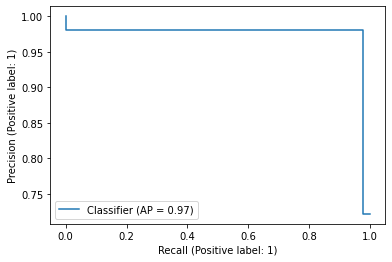
\includegraphics[width=.50\textwidth]{../models_performance_graphs/ptb/transformer_ptb_auprc.png}\hfill
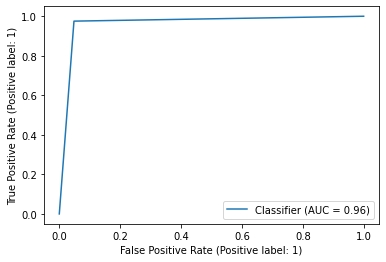
\includegraphics[width=.50\textwidth]{../models_performance_graphs/ptb/transformer_ptb_auroc.png}\hfill
\caption{(left) AURPC curve of the CNN with residual blocks for the PTB dataset. \\ (right) AUROC curve of the CNN with residual blocks for the PTB dataset}
\label{fig:transformer_ptb_two}
\end{figure}











































%%%%%%%%%%%%%%%%%%%%%%%%%%%%%%%%%%%%% ENSEMBLE %%%%%%%%%%%%%%%%%%%%%%%%%%%%%%%%%%%%%%%%%%%%%%%%%%
\section{Ensemble of models}

%%%%%%% ENSEMBLE ONE %%%%%%%
\subsection{Average of the outputs}
%%%%%%% MIT %%%%%%%
\subsubsection{MIT\_BIH}

%%%%%%% PTB %%%%%%%
\subsubsection{PTB}

%%%%%%% ENSEMBLE TWO %%%%%%%
\subsection{Logistic regression on the outputs}
%%%%%%% MIT %%%%%%%
\subsubsection{MIT\_BIH}

%%%%%%% PTB %%%%%%%
\subsubsection{PTB}

\end{document}
